\documentclass[../main.tex]{subfiles}
\begin{document}
\section{轨迹规划}

\subsection{轨迹规划的基本概念}
\begin{enumerate}
    \item \textbf{轨迹规划}:用一定的\textbf{函数形式}表示控制量(位置、速度、加速度)的\textbf{控制律},根据\textbf{约束或/和最优目标},求取控制律\textbf{参数}。
    \item \textbf{目标}:给定路径与约束,生成一组控制序列,使机器人从初始位姿移动到目标位姿。
    \item \textbf{关节式机器人轨迹规划}:
        \begin{itemize}
            \item \textbf{末端轨迹规划}:得到末端在笛卡尔空间中的位置、速度、加速度控制序列
            \item \textbf{关节轨迹规划}:得到关节空间中的角度、角速度和角加速度控制序列
        \end{itemize}
    \item \textbf{核心过程}:
        \begin{itemize}
            \item \textbf{控制律}:采用一定的\textbf{函数}形式表示控制量(位置/速度/加速度)的控制律
            \item \textbf{约束}:
                \begin{enumerate}
                    \item 路径约束
                    \item 运动学约束
                        \begin{enumerate}
                            \item 最大速度、最大加速度(非完整运动学约束)
                            \item 最小转弯半径
                        \end{enumerate}
                    \item 边界约束
                        \begin{enumerate}
                            \item 初始状态(位置、速度、加速度)\footnote{位置给定,速度、加速度一般给定为0}
                            \item 终点状态(位置、速度、加速度)\footnote{位置给定,速度、加速度一般给定为0}
                            \item 中间状态(部分问题)
                        \end{enumerate}                    
                    \item 连续性/光滑性要求\footnote{路径得到的是直线段,如果完全按照直线段执行,对于存在非完整运动学约束的机器人来讲,无法实现流畅运动,\textbf{移动效率低};通过\textbf{轨迹平滑}可以减少因为方向变化而花费的启停时间、以及因方向突变而导致的底盘打滑问题}\footnote{速度连续属于\textbf{一阶平滑},加速度连续也就是速度平滑属于\textbf{二阶平滑}}
                    \item 无碰约束
                \end{enumerate}
            \item \textbf{求参}:根据约束或/和最优目标,求取控制律\textbf{函数参数}
        \end{itemize}
    \item \textbf{主要方法}:
        \begin{itemize}
            % 与下方目录对应的新链接(指向下面新增的锚点)
            \item \hyperref[sec:1d-poly]{一维轨迹规划}
                \begin{itemize}
                    \item \hyperref[sec:basic-1d]{基本一维轨迹规划}
                        \begin{itemize}
                            \item \hyperref[method:poly]{多项式}
                        \end{itemize}
                    \item \hyperref[sec:composite-1d]{复合一维轨迹规划}
                    \begin{itemize}
                        \item \hyperref[method:parabola]{抛物线轨迹}
                        \item \hyperref[method:trapezoid]{梯形速度轨迹}
                        \item \hyperref[method:doubleS]{双S速度曲线}
                    \end{itemize}
                \end{itemize}
            \item \hyperref[sec:planar]{移动机器人平面轨迹规划}
                \begin{itemize}
                    \item \hyperref[method:graph]{图形搜索法}
                    \item \hyperref[method:opt]{参数优化法}
                    \item \hyperref[method:feedback]{反馈控制法}
                \end{itemize}
        \end{itemize}
\end{enumerate}

% ===================== 目录对应的正文(每个方法均有锚点/label) =====================

\subsection{一维轨迹规划(多项式)}\label{sec:1d-poly}
\textbf{常用形式}:多项式、三角函数、指数函数

\textbf{阶数的选取}:\\
    {\small\kaishu
    \textbf{例题:一维多项式轨迹规划示例}
    
    已知:
    \[
    t_0 = 0, \quad t_1 = 10
    \]
    \[
    q_0 = q(t_0) = 10, \quad q_1 = q(t_1) = 20
    \]
    \[
    v_0 = v(t_0) = 0, \quad v_1 = v(t_1) = 0
    \]
    \[
    v(t=2) = 2, \quad a(t=8) = 0
    \]
    
    求:该轨迹至少需要几阶多项式表示?
    
    选项:
    \begin{itemize}
        \item[(A)] 4
        \item[(B)] 5
        \item[(C)] 6
        \item[(D)] 7
    \end{itemize}
    
    \vspace{1em}
    \textbf{解析:}
    
    共有六个约束条件:
    \begin{enumerate}
        \item $q(t_0) = 10$
        \item $q(t_1) = 20$
        \item $v(t_0) = 0$
        \item $v(t_1) = 0$
        \item $v(t=2) = 2$
        \item $a(t=8) = 0$
    \end{enumerate}
    
    若设轨迹为 $q(t) = a_0 + a_1 t + a_2 t^2 + a_3 t^3 + a_4 t^4 + a_5 t^5$,  
    则其一阶、二阶导数为:
    \[
    \dot{q}(t) = a_1 + 2a_2 t + 3a_3 t^2 + 4a_4 t^3 + 5a_5 t^4
    \]
    \[
    \ddot{q}(t) = 2a_2 + 6a_3 t + 12a_4 t^2 + 20a_5 t^3
    \]
    
    六个约束需要解六个未知数 $a_0,a_1,a_2,a_3,a_4,a_5$,  
    因此多项式的最高次项应为 $t^5$,五阶多项式。
    
    \vspace{0.5em}
    \textbf{答案:} (B) 5
    }
\begin{enumerate}
    \item \textbf{基本一维轨迹规划}\label{sec:basic-1d}
        \begin{enumerate}
            \item \textbf{多项式}\label{method:poly}
                \begin{itemize}
                    \item \textbf{一阶多项式(位置连续)}\\
                    {\small\kaishu
                    设 $T=t_1-t_0,\ h=q_1-q_0$,取
                    \[
                    q(t)=a_0+a_1 t = q_0+\frac{h}{T}(t-t_0),\quad
                    \dot q(t)=\frac{h}{T},\quad
                    \ddot q(t)=0 .
                    \]
                    亦可写成矩阵方程
                    \[
                    \begin{bmatrix}1&0\\ 1&T\end{bmatrix}
                    \begin{bmatrix}a_0\\ a_1\end{bmatrix}
                    =\begin{bmatrix}q_0\\ q_1\end{bmatrix},\quad a_0=q_0,\ a_1=\frac{h}{T}.
                    \]
                    }
                    \item \textbf{三阶多项式(位置、速度连续)}\\
                    {\small\kaishu
                    可同时满足任意的 $q_0,q_1,v_0,v_1$ 约束。令 $\tau=t-t_0,\ T=t_1-t_0,\ h=q_1-q_0$,
                    \[
                    q(t)=a_0+a_1\tau+a_2\tau^2+a_3\tau^3,
                    \]
                    其中
                    \[
                    a_0=q_0,\quad a_1=v_0,\quad
                    a_2=\frac{3h-(2v_0+v_1)T}{T^2},\quad
                    a_3=\frac{-2h+(v_0+v_1)T}{T^3}.
                    \]
                    \begin{itemize}
                        \item \textbf{给定中间点速度}:在每个小区间 $[t_k,t_{k+1}]$ 指定 $q_k,q_{k+1}$ 与端点速度 $v_k,v_{k+1}$\footnote{多点轨迹可用多段三次多项式拼接实现}
                        \item \textbf{未给定中间点速度}:可用启发式
                    \[
                    v_k=\begin{cases}
                    0,& \mathrm{sign}(d_k)\neq \mathrm{sign}(d_{k+1}),\\[2pt]
                    \tfrac12(d_k+d_{k+1}),& \mathrm{sign}(d_k)=\mathrm{sign}(d_{k+1}),
                    \end{cases}
                    \quad
                    d_k=\dfrac{q_k-q_{k-1}}{t_k-t_{k-1}}.
                    \]
                    三次拼接保证 $q,\dot q$ 连续($C^1$),但一般\emph{不能}保证 $\ddot q$ 连续。
                    \end{itemize}
                    }
                    \begin{figure}[H]
                        \centering
                        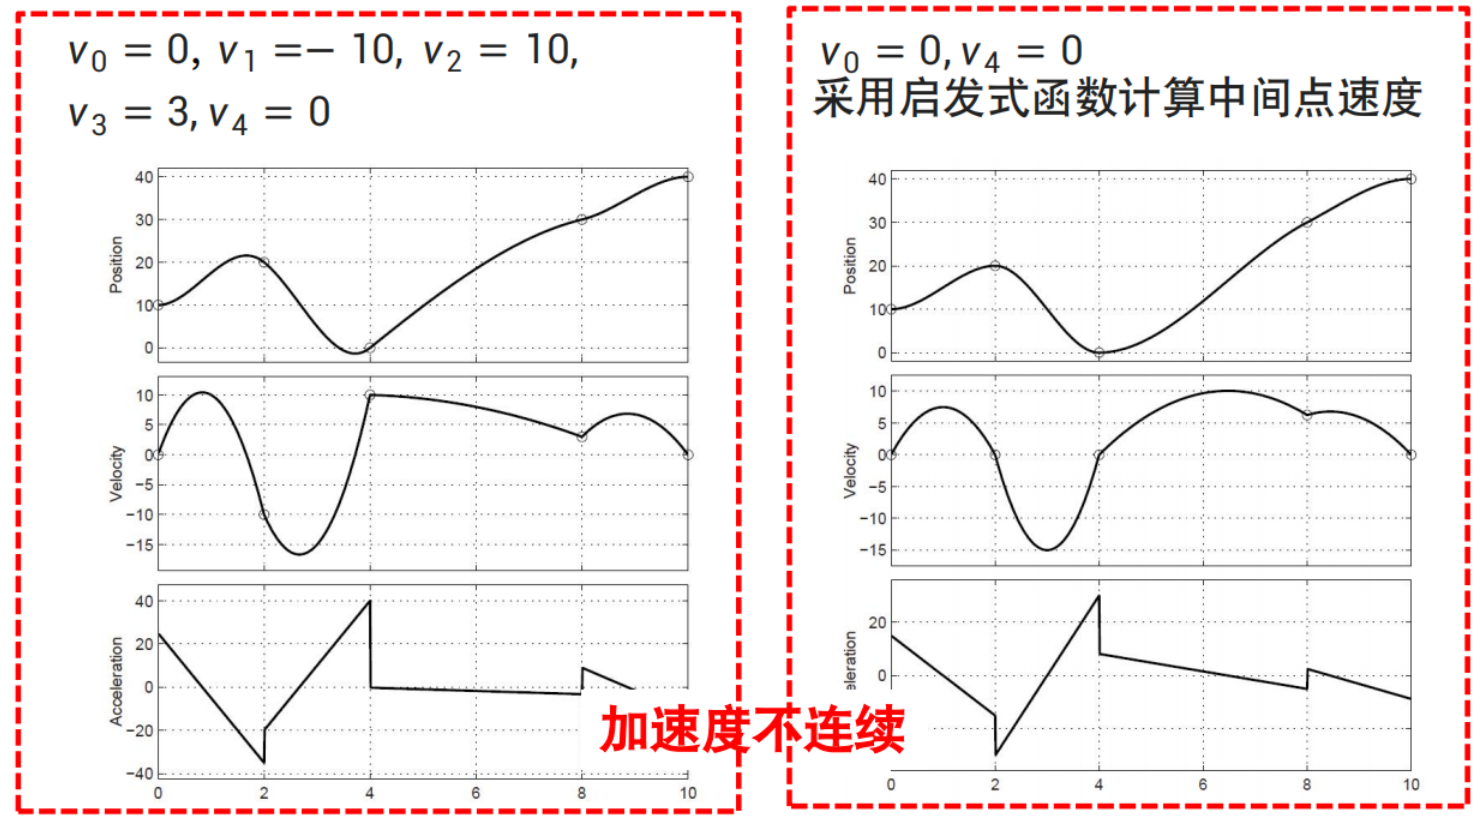
\includegraphics[width=0.6\textwidth]{images/3jie.png}
                        \caption{三阶多项式曲线(给定 vs 启发式)}
                    \end{figure}    
                    \item \textbf{五阶多项式(位置、速度、加速度连续)}\\
                    {\small\kaishu
                    可同时满足 $q_0,q_1,v_0,v_1,\ddot q_0,\ddot q_1$ 六个端点约束,从而在多段拼接时实现加速度连续($C^2$)。
                    令 $\tau=t-t_0,\ T=t_1-t_0$,取
                    \[
                    q(t)=q_0+v_0\tau+\tfrac12\ddot q_0\,\tau^2+b_3\tau^3+b_4\tau^4+b_5\tau^5,
                    \]
                    其中系数为
                    \[
                    b_3=\frac{-3T^2\ddot q_0+T^2\ddot q_1-12Tv_0-8Tv_1-20q_0+20q_1}{2T^3},
                    \]
                    \[
                    b_4=\frac{\tfrac32T^2\ddot q_0-T^2\ddot q_1+8Tv_0+7Tv_1+15q_0-15q_1}{T^4},
                    \]
                    \[
                    b_5=\frac{-T^2\ddot q_0+T^2\ddot q_1-6Tv_0-6Tv_1-12q_0+12q_1}{2T^5}.
                    \]
                    (多段五次多项式常用于多点轨迹,保证位置、速度、加速度在拼接处连续。)
                    }
                    
                    \item \textbf{七阶多项式(位置、速度、加速度、加加速度连续)}\\
                    \begin{figure}[htbp]
                        \centering
                        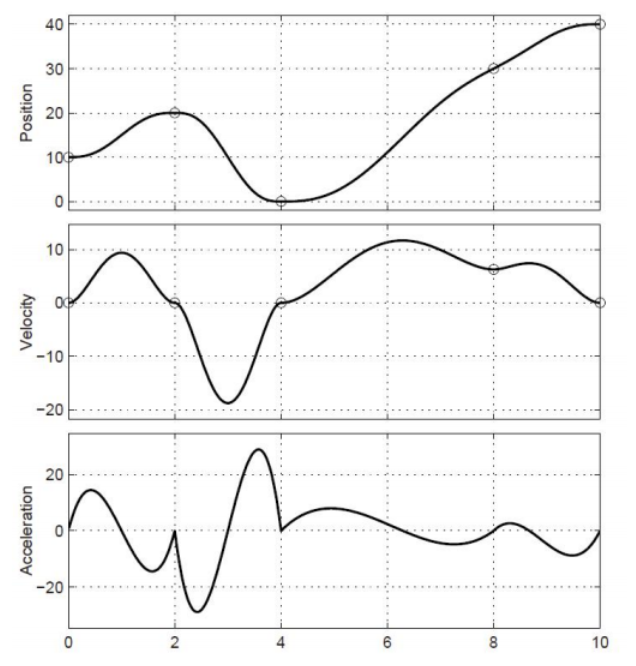
\includegraphics[width=0.35\textwidth]{images/5jie.png}
                        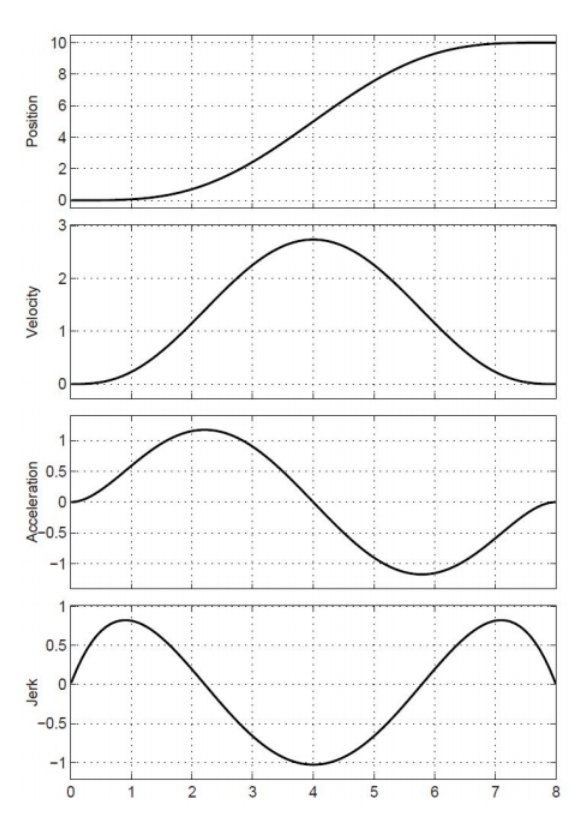
\includegraphics[width=0.26\textwidth]{images/7jie.png}
                        \caption{五阶、七阶多项式曲线}
                        \label{fig:bug2bad}
                    \end{figure}
                \end{itemize}
        \end{enumerate}

    \item \textbf{复合一维轨迹规划}\label{sec:composite-1d}
        \begin{enumerate}
            \item \textbf{抛物线轨迹}\label{method:parabola}
                    \begin{figure}[H]
                        \centering
                        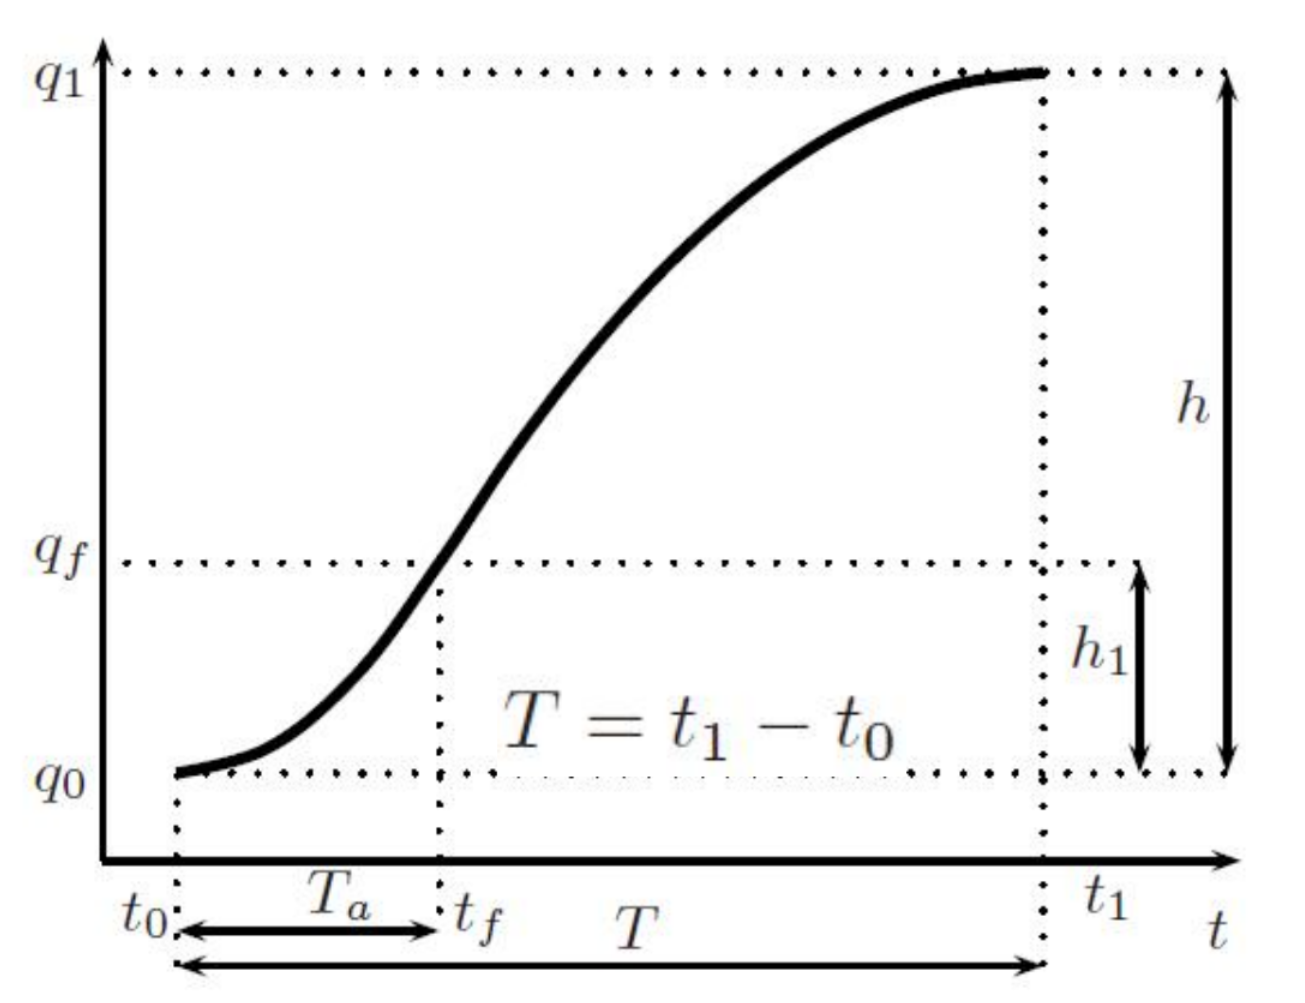
\includegraphics[width=0.4\textwidth]{images/pwx0.png}
                        \caption{抛物线轨迹图}
                    \end{figure}    
            {\small\kaishu
            \begin{itemize}
                \item \textbf{基本思想:}  
                由两个二次多项式拼接而成,加速度恒定但方向相反,形成加速—减速的“抛物线”位移曲线,可同时满足初末位置与初末速度约束。
                \[
                \begin{cases}
                q_a(t) = a_0 + a_1(t-t_0) + a_2(t-t_0)^2, & t\in[t_0,t_f],\\[4pt]
                q_b(t) = a_3 + a_4(t-t_0) + a_5(t-t_0)^2, & t\in[t_f,t_1].
                \end{cases}
                \]
                其中 $t_f$ 为中间切换时刻,$T=t_1-t_0$。\\
                \textcolor{red}{接下来分三种情况:\;①时间与位置都对称;②\textbf{时间对称但位置不对称}(保持 $t_f=\tfrac{t_0+t_1}{2}$,取消 $q_f=\tfrac{q_0+q_1}{2}$);③时间与位置均不对称,分别讨论如何求解$a_1,a_2,a_3,a_4,a_5,a_6$}\\================================   
                \item \textbf{情况一:若要求时间、轨迹都对称,即$t_f=(t_0+t_1)/2$,$q_f=(q_0+q_1)/2$:}
                \begin{enumerate}
                    \item 阶段1(加速段, $t\in[t_0,t_f]$):
                    \[
                    \begin{cases}
                    q_a(t_0)=q_0=a_0,\\
                    \dot q_a(t_0)=v_0=a_1,\\
                    q_a(t_f)=q_f=a_0+a_1(t_f-t_0)+a_2(t_f-t_0)^2.
                    \end{cases}
                    \]
                    由此得
                    \[
                    a_0=q_0,\quad a_1=v_0,\quad a_2=\frac{2(h-v_0T)}{T^2},\quad h=q_1-q_0.
                    \]
        
                    \item 阶段2(减速段, $t\in[t_f,t_1]$):
                    \[
                    \begin{cases}
                    q_b(t_f)=q_f=a_3,\\
                    q_b(t_1)=q_1=a_3+a_4(t_1-t_f)+a_5(t_1-t_f)^2,\\
                    \dot q_b(t_1)=v_1=a_4+2a_5(t_1-t_f).
                    \end{cases}
                    \]
                    若轨迹对称,则
                    \[
                    t_f=\frac{t_0+t_1}{2},\quad q_f=\frac{q_0+q_1}{2},
                    \]
                    从而
                    \[
                    a_3=q_f,\quad a_4=2\frac{h}{T}-v_1,\quad a_5=\frac{2}{T^2}(v_1T-h).
                    \]

                    \item \textbf{始末速度:}
                        \begin{itemize}
                            \item 若 $v_0=v_1$,则在 $t_f$ 处速度连续;
                            \item 若 $v_0\neq v_1$,则在 $t_f$ 处速度不连续;
                        \end{itemize}
                \end{enumerate}
            ================================   
             \item \textbf{情况二:若要求时间对称,不要求轨迹对称,即$t_f=(t_0+t_1)/2$,$q_f\neq(q_0+q_1)/2$:}
             \\可由以下方程解得$a_1,a_2,a_3,a_4,a_5,a_6$
            \( \left\{  \begin{array}{l} {\dot{q}}_{a}\left( {t}_{0}\right)  = {a}_{1} = {v}_{0} \\  {\dot{q}}_{a}\left( {t}_{0}\right)  = {a}_{1} = {v}_{0} \\  {q}_{b}\left( {t}_{1}\right)  = {a}_{3} + {a}_{4}\frac{T}{2} + {a}_{5}{\left( \frac{T}{2}\right) }^{2} = {q}_{1} \\  {\dot{q}}_{b}\left( {t}_{1}\right)  = {a}_{4} + 2{a}_{5}\frac{T}{2} = {v}_{1} \\  {q}_{a}\left( {t}_{f}\right)  = {a}_{0} + {a}_{1}\frac{T}{2} + {a}_{2}{\left( \frac{T}{2}\right) }^{2} = {a}_{3} = {q}_{b}\left( t_f\right) \\  {\dot{q}}_{a}\left( {t}_{f}\right)  = {a}_{1} + 2{a}_{2}\frac{T}{2} = {a}_{4} = {\dot{q}}_{b}\left( {t}_{f}\right)  \end{array}\right. \)
            其中 \( \frac{T}{2} = \left( {{t}_{f} - {t}_{0}}\right)  = \left( {{t}_{1} - {t}_{f}}\right) \)
            \\================================   
             \item \textbf{情况三:若不要求时间、轨迹对称,即$t_f\neq(t_0+t_1)/2$,$q_f\neq(q_0+q_1)/2$:}             
            \\可由以下方程解得$a_1,a_2,a_3,a_4,a_5,a_6$
             \( \left\{  \begin{array}{l} {q}_{a}\left( {t}_{0}\right)  = {a}_{0} = {q}_{0} \\  {\dot{q}}_{a}\left( {t}_{0}\right)  = {a}_{1} = {v}_{0} \\  {q}_{b}\left( {t}_{1}\right)  = {a}_{3} + {a}_{4}\left( {{t}_{1} - {t}_{f}}\right)  + {a}_{5}{\left( {t}_{1} - {t}_{f}\right) }^{2} = {q}_{1} \\  {\dot{q}}_{b}\left( {t}_{1}\right)  = {a}_{4} + 2{a}_{5}\left( {{t}_{1} - {t}_{f}}\right)  = {v}_{1} \\  {q}_{a}\left( {t}_{f}\right)  = {a}_{0} + {a}_{1}\left( {{t}_{1} - {t}_{f}}\right)  + {a}_{2}{\left( {t}_{1} - {t}_{f}\right) }^{2} = {a}_{3}\left( { = {q}_{b}\left( {t}_{f}\right) }\right. \\  \left. {{\dot{q}}_{a}\left( {t}_{f}\right)  = {a}_{1} + 2{a}_{2}\left( {{t}_{1} - {t}_{f}}\right) }\right)  = {a}_{4}\left( { = {\dot{q}}_{b}\left( {t}_{f}\right) }\right)  \end{array}\right. \)
            \\$t_f$ 作为自由变量,最后参数和其取值有关,根据最大加速度或任务约束优化确定。
            \\================================   
            \item \textcolor{red}{为什么若想分段中间点满足位置和速度的连续性要求,必须取消中间位置约束,即要求轨迹不对称?}
            
            {\small\kaishu
            抛物线轨迹由两段二次多项式组成:
            \[
            \begin{cases}
            q_a(t) = a_0 + a_1(t - t_0) + a_2(t - t_0)^2, & t\in[t_0, t_f],\\[4pt]
            q_b(t) = a_3 + a_4(t - t_f) + a_5(t - t_f)^2, & t\in[t_f, t_1].
            \end{cases}
            \]
            共有六个未知参数 $a_0,a_1,a_2,a_3,a_4,a_5$。  
            若要求轨迹在中间点 $t_f$ 处位置与速度连续,可列出六个约束:
            \[
            \begin{cases}
            q_a(t_0)=q_0, \quad \dot q_a(t_0)=v_0,\\
            q_b(t_1)=q_1, \quad \dot q_b(t_1)=v_1,\\
            q_a(t_f)=q_b(t_f), \quad \dot q_a(t_f)=\dot q_b(t_f),
            \end{cases}
            \]
            方程数与未知数相等,恰可求解。  
            
            若再强制轨迹“对称”,即:
            \[
            q_f=\frac{q_0+q_1}{2},
            \]
            则系统多出一个额外条件,约束数变为七个而未知数仍为六个,方程组过约束,无法同时满足。  
            
            因此,若希望轨迹在中间点既满足位置又满足速度连续,必须取消中间位置约束 $q_f$,
            使轨迹自动调整中点高度,即形成不对称轨迹。
            }

            \end{itemize}
            }
            \begin{figure}[htbp]
                \centering
                % 第一行
                \begin{subfigure}{0.32\textwidth}
                    \centering
                    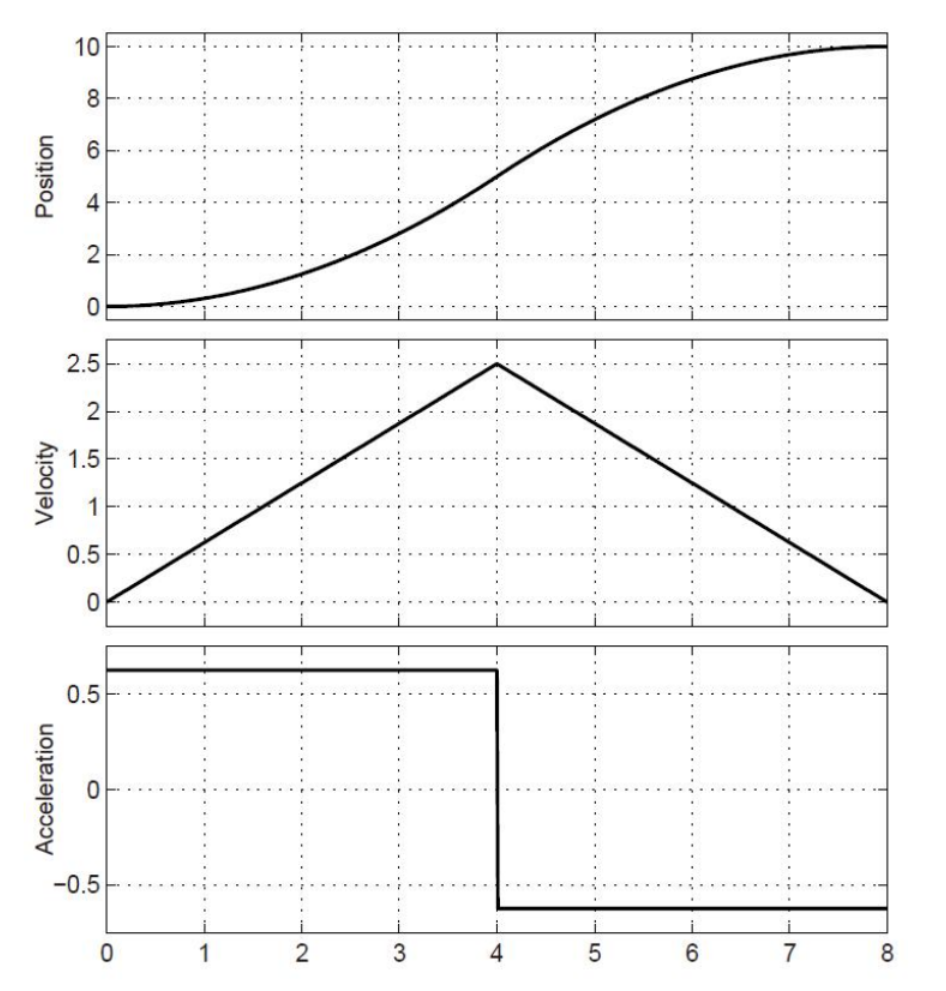
\includegraphics[width=\linewidth]{images/pwx1.png}
                    \caption{初末速度不等,对称时间、对称轨迹}
                    \label{fig:pwx1}
                \end{subfigure}
                \begin{subfigure}{0.32\textwidth}
                    \centering
                    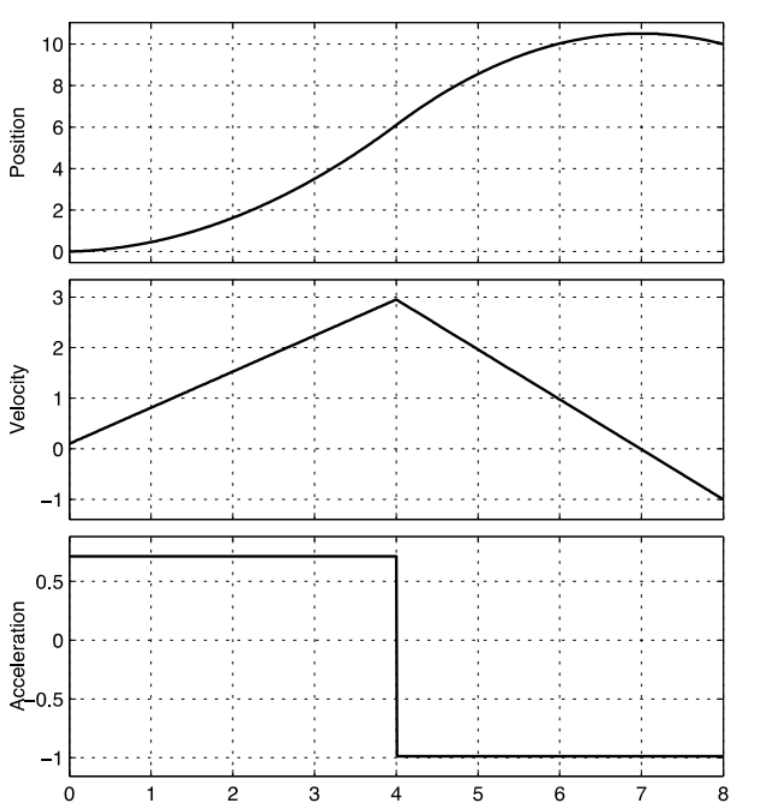
\includegraphics[width=\linewidth]{images/pwx2.png}
                    \caption{初末速度不等,对称时间、非对称轨迹}
                    \label{fig:pwx2}
                \end{subfigure}
                \begin{subfigure}{0.32\textwidth}
                    \centering
                    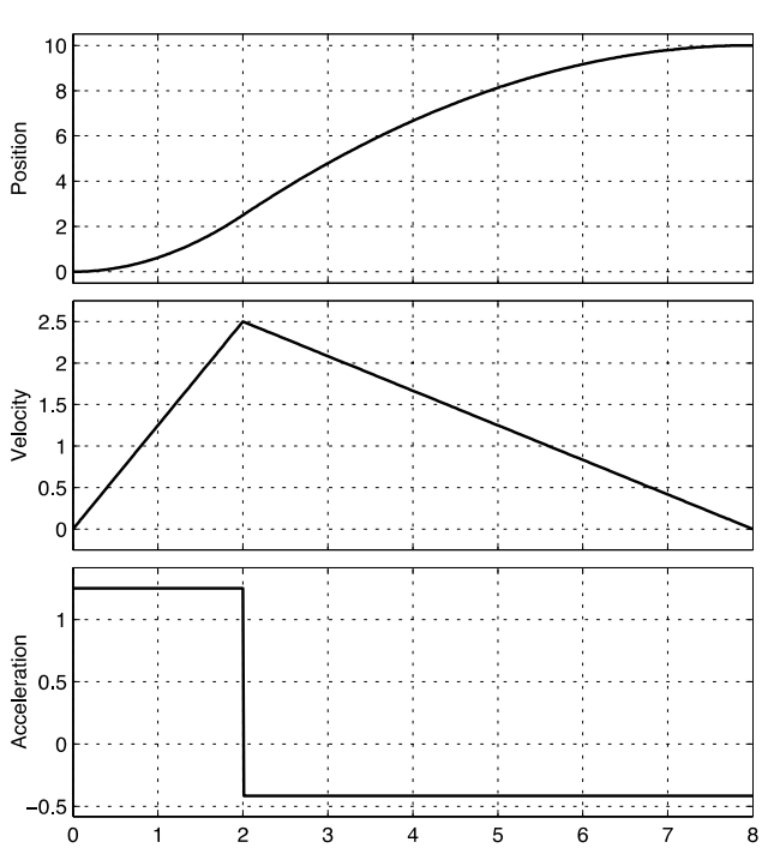
\includegraphics[width=\linewidth]{images/pwx3.png}
                    \caption{初末速度不等,非对称时间、非对称轨迹}
                    \label{fig:pwx3}
                \end{subfigure}
            \end{figure}
            \item \textbf{梯形速度轨迹}\label{method:trapezoid}
            {\small\kaishu
            \begin{itemize}
                \item \textbf{基本思想:}  
                梯形速度轨迹由两个二阶多项式和一个一阶多项式合成,
                分为加速、匀速、减速三段:
                \[
                \begin{cases}
                \text{加速段 } t\in[0,T_a]: &
                \begin{cases}
                q(t)=a_0+a_1t+a_2t^2,\\
                \dot q(t)=a_1+2a_2t,\\
                \ddot q(t)=2a_2;
                \end{cases}\\[6pt]
                \text{匀速段 } t\in[T_a,\,t_1-T_d]: &
                \begin{cases}
                q(t)=b_0+b_1t,\\
                \dot q(t)=b_1=v_c,\\
                \ddot q(t)=0;
                \end{cases}\\[6pt]
                \text{减速段 } t\in[t_1-T_d,\,t_1]: &
                \begin{cases}
                q(t)=c_0+c_1t+c_2t^2,\\
                \dot q(t)=c_1+2c_2t,\\
                \ddot q(t)=2c_2.
                \end{cases}
                \end{cases}
                \]
                给定 $q_0,q_1,v_0,v_1$,以及匀速段速度 $v_c$,
                即可确定各段参数。
                \begin{figure}[H]
                    \centering
                    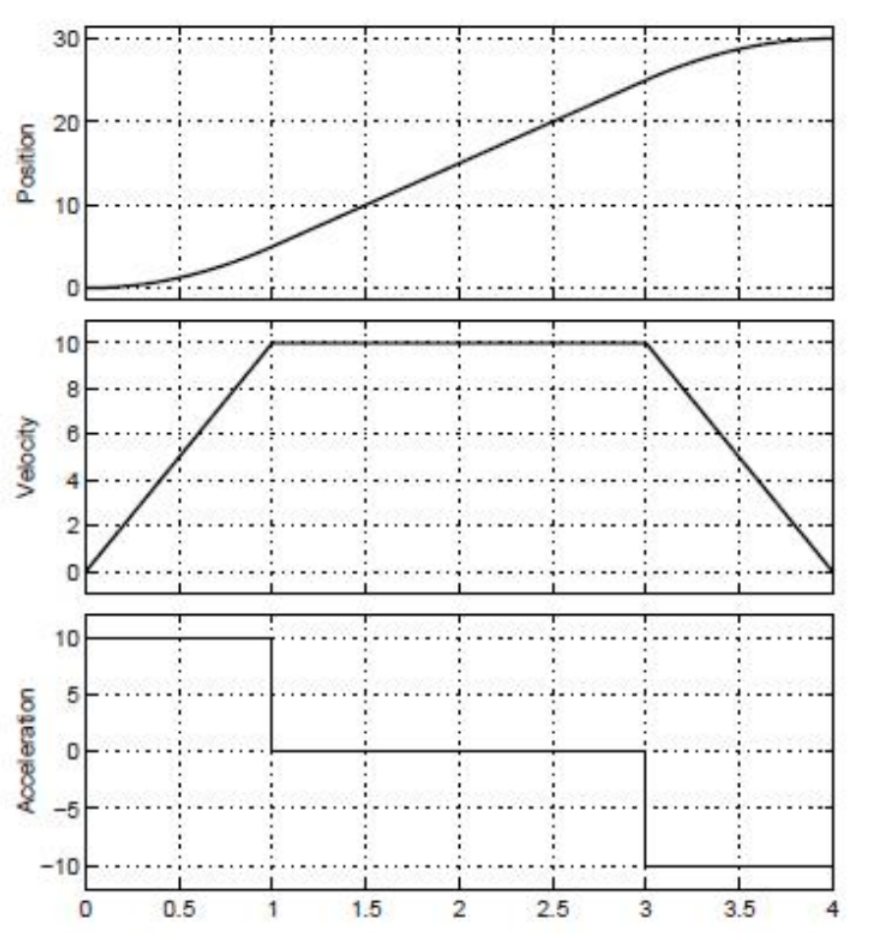
\includegraphics[width=0.43\textwidth]{images/tx.png}
                    \caption{梯形轨迹图}
                \end{figure}   
                \item \textbf{可行轨迹:}
                \begin{itemize}
                    \item[(1)] \textbf{检查是否存在可行轨迹:}
                    \[
                    a_{\max} < \frac{|v_0^2 - v_1^2|}{2|q_1 - q_0|}
                    \quad \Rightarrow \quad \text{轨迹不可行。}
                    \]
                    \textcolor{red}{若 $v_0=v_1=0$,则总能找到可行轨迹}
                    
                    \vspace{0.5em}
                \item[(2)] \textbf{可行且可加速至 $v_c=v_{\max}$:}
                \[
                T_a = \frac{v_{\max}-v_0}{a_{\max}}, \quad
                T_d = \frac{v_{\max}-v_1}{a_{\max}},
                \]
                \[
                T = \frac{h}{v_{\max}}
                + \frac{v_{\max}}{2a_{\max}}\left(1-\frac{v_0}{v_{\max}}\right)^2
                + \frac{v_{\max}}{2a_{\max}}\left(1-\frac{v_1}{v_{\max}}\right)^2,
                \quad h=q_1-q_0.
                \]
                
                {\footnotesize
                其中:
                $T_a$ 为加速时间,$T_d$ 为减速时间,$T$ 为总运动时间,
                $h=q_1-q_0$ 为总位移;
                $v_0,v_1$ 分别为初始与末端速度,
                $v_{\max}$ 为最大允许速度,
                $a_{\max}$ 为最大加速度。
                }
                
                \vspace{0.5em}
                
                \item[(3)] \textbf{可行但无法达到 $v_{\max}$(无匀速段):}
                \[
                v_c = v_{\lim} = 
                \sqrt{h a_{\max} + \frac{v_0^2 + v_1^2}{2}} < v_{\max},
                \]
                \[
                T_a = \frac{v_{\lim}-v_0}{a_{\max}}, \quad
                T_d = \frac{v_{\lim}-v_1}{a_{\max}}, \quad
                T = T_a + T_d.
                \]
                
                {\footnotesize
                其中:
                $v_{\lim}$ 为在加速、减速段相接时的极限速度(最大可达匀速速度);
                $T_a,T_d,T$、$v_0,v_1,a_{\max},h$ 含义同上。
                }
                \end{itemize}
                
                \vspace{0.5em}
                \item \textbf{特点:}
                \begin{itemize}
                    \item 实现最小时间的方式:通过以最大加速度加速至 $v_c$,再以最大减速度减速;
                    \item 问题:虽然速度连续,但加速度存在\textbf{不连续阶跃},
                    即 $jerk$ 为无穷大,
                    在加速—匀速、匀速—减速交界处会产生冲击或振动。
                \end{itemize}
            \end{itemize}
            }

            \item \textbf{双S速度曲线}\label{method:doubleS}
                \begin{figure}[H]
                    \centering
                    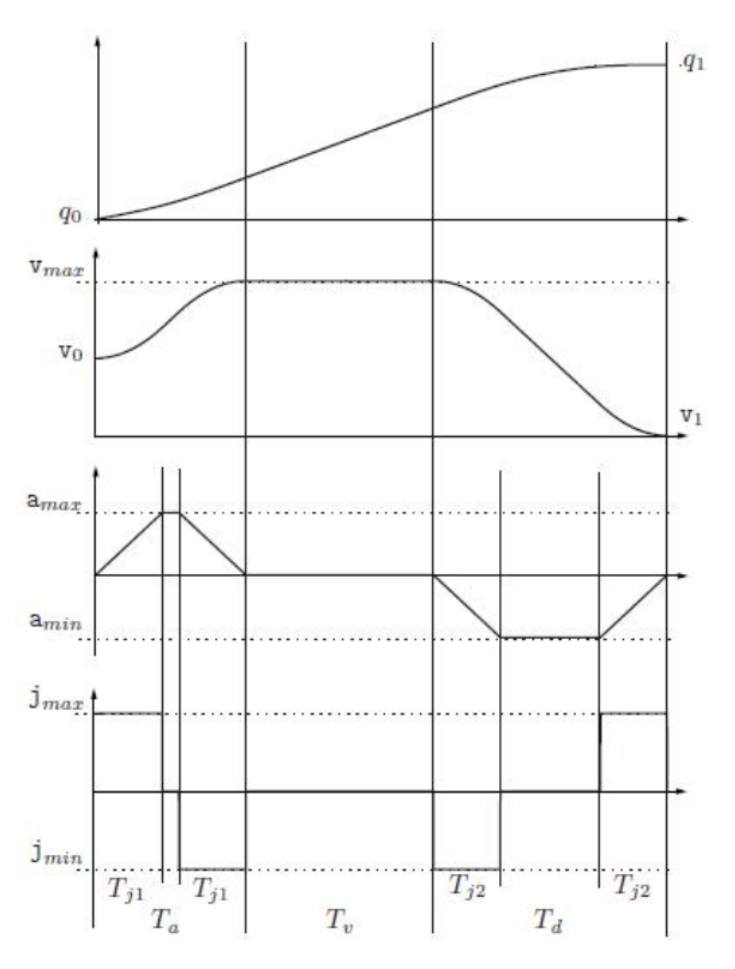
\includegraphics[width=0.43\textwidth]{images/doubleS.png}
                    \caption{双S速度曲线图}
                \end{figure} 
                \begin{itemize}
                {\small\kaishu
                \item \textbf{每段采用多项式:}\\
                双S速度轨迹由 7 段(加速 3 段 + 匀速 1 段 + 减速 3 段)组成
                \begin{enumerate}
                    \item \emph{恒加加速度段}($j(t)=\pm j_{\max}$,时长 $T_{j1},T_{j2}$ ):
                    \[
                    \begin{aligned}
                    a(t) &= a_0 + j\,t,\\
                    v(t) &= v_0 + a_0 t + \tfrac12 j t^2,\\
                    q(t) &= q_0 + v_0 t + \tfrac12 a_0 t^2 + \tfrac16 j t^3
                    \end{aligned}
                    \]
                    (加速度线性、速度二次、位置三次)
                    \item \emph{恒加速度段}($j(t)=0,\ a(t)=\pm a_{\max}$,时长 $T_a,T_d$):
                    \[
                    v(t)=v_0+a\,t,\qquad
                    q(t)=q_0+v_0 t+\tfrac12 a t^2
                    \]
                    (速度一次、位置二次)
                    \item \emph{恒速度段}($a(t)=0,\ v(t)=v_c$,时长 $T_v$):
                    \[
                    q(t)=q_0+v_c t
                    \]
                    (位置一次)
                \end{enumerate}
                以上三类段按“加速-匀速-减速”依次拼接,构成速度呈双S形的剖面。
                
            
                \item 经典双S在各段交界处 \emph{jerk} 为阶跃(不连续)。若需 \emph{jerk} 连续($C^3$ 连续轨迹),可采用:
                \begin{itemize}
                    \item 使用单段或分段七阶多项式,在端点同时约束 $q,v,a,j$(共 8 个约束),从而使 $q(t)$ 达到 $C^3$ 连续;
                \end{itemize}
                }
            \end{itemize}
        \end{enumerate}
        \textbf{小结}
        \begin{table}[htbp]
        \centering
        \caption{\centering
        常见一维轨迹形式的连续性与多项式阶次对比\\($^\ast$时间对称、轨迹不对称的情况下可以使速度连续)}
        \begin{tabular}{lcccc}
        \toprule
        方法 & 位置曲线最高次幂 & 速度是否连续 & 加速度是否连续 & 加加速度是否连续 \\
        \midrule
        抛物线轨迹 & 2 & ×$^\ast$ & × & × \\
        梯形速度轨迹 & 2 & √ & × & × \\
        双S速度曲线 & 3 & √ & √ & × \\
        \bottomrule
        \end{tabular}
        \end{table}
\end{enumerate}



\subsection{移动机器人平面轨迹规划}\label{sec:planar}
\begin{itemize}
    \item \textbf{平面轨迹规划}:二维轨迹规划$(x(t),y(t))$或$(v(t),\omega(t))$\footnote{在平面上移动时,机器人有三个状态量$(x,y,\theta)$,理论上应该做三维轨迹规划$(x(t),y(t),\theta(t))$,但由于\( \theta \left( t\right)  = \operatorname{actan}\frac{\dot{y}\left( t\right) }{\dot{x}\left( t\right) } = \operatorname{actan}\frac{y\left( {t + 1}\right)  - y\left( t\right) }{x\left( {t + 1}\right)  - x\left( t\right) } \) 且\( \dot{\theta }\left( t\right)  = w\left( t\right) \) \( \ \dot{x}\left( t\right)  = v\left( t\right) \cos \theta \left( t\right) \) \( \dot{y}\left( t\right)  = v\left( t\right) \sin \theta \left( t\right) \),即由基本的二维轨迹可以还原成完整的三维轨迹}
    \item \textbf{方法分类}:
        \begin{itemize}
            \item $(x(t),y(t))$:
                \begin{itemize}
                    \item 完整机器人:独立规划、时间同步
                    \item 非完整机器人:图形搜索法
                \end{itemize}
            \item $(v(t),\omega(t))$:
                \begin{itemize}
                    \item 参数优化法、反馈控制法
                \end{itemize}
        \end{itemize}
\end{itemize}
\begin{enumerate}
    \item \textbf{图形搜索法}\label{method:graph}
        \begin{itemize}
            \item \textbf{主要思路}:根据路径搜索经过或者近似经过路径点且满足运动学约束的图形曲线
            \item \textbf{基本思想}:采用\textbf{运动基元},从起始点开始不断搜索由\textbf{运动基元组合}而成的\textbf{最佳单词}来获得最优轨迹
            \textbf{优点}:
                \begin{itemize}
                    \item 可以实现\textbf{位置}的连续平滑,并充分考虑了机器人的\textbf{运动学约束}和\textbf{时间最优要求}
                \end{itemize}
            \textbf{缺点}:
                \begin{itemize}
                    \item \textbf{最佳单词}:如何构建单词和搜索最佳单词
                    \item \textbf{空间分辨率降低}:运动基元方式实际是对状态空间和/或控制空间进行了离散化,直接导致空间分辨率降低,能达到的边界状态只是预定义单词能够达到的状态
                \end{itemize}                
             \textbf{常见曲线}:Dubins曲线、Reeds-Shepp曲线、Balkcom-Mason曲线、回旋曲线、多项式曲线、贝塞尔曲线、样条曲线等
                \begin{enumerate}
                    \item \textbf{DUBINS曲线}
                            \begin{figure}[H]
                                \centering
                                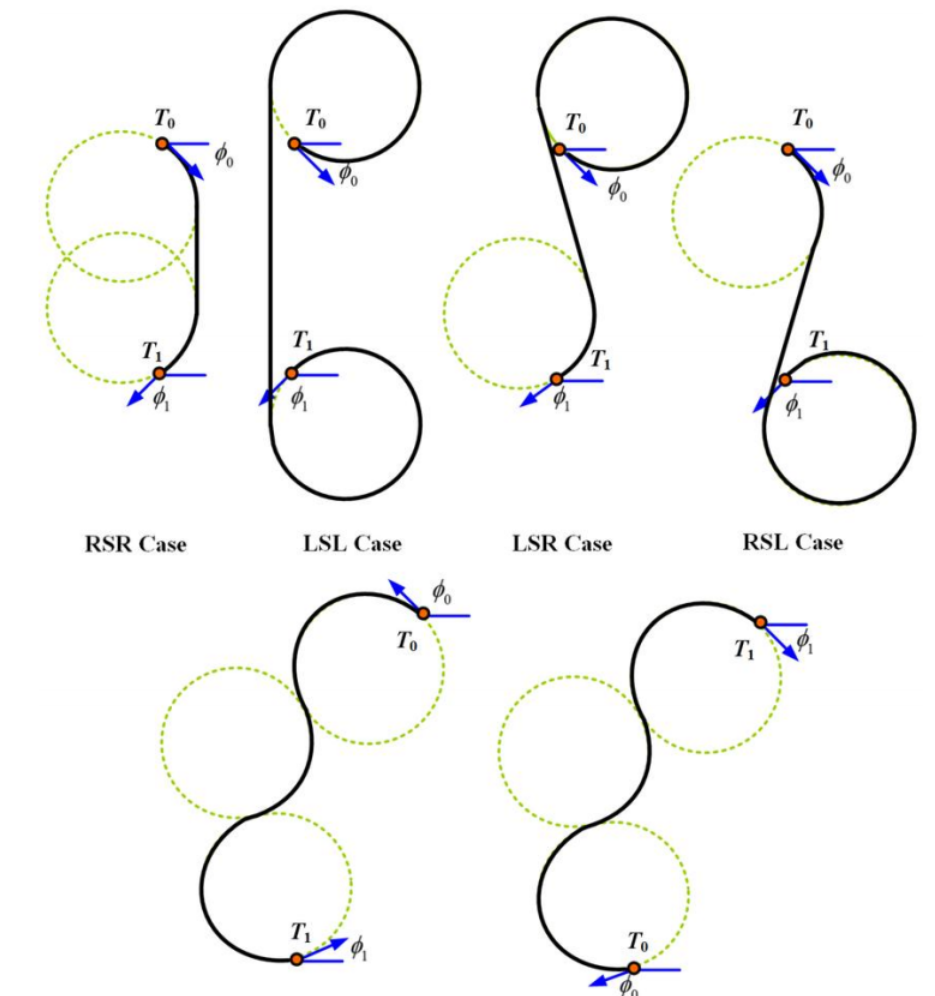
\includegraphics[width=0.43\textwidth]{images/DUBINS.png}
                                \caption{DUBINS曲线}
                            \end{figure} 
                        \begin{itemize}
                            \item \textbf{系统方程}:
                            \[
                            \text{} \quad
                            \begin{cases}
                            \dot{x} = \cos\theta, \\[4pt]
                            \dot{y} = \sin\theta, \\[4pt]
                            \dot{\theta} = u_{\phi},
                            \end{cases}
                            \qquad
                            u_{\phi} \in \left[-\dfrac{1}{L}\tan\phi_{\max},\; \dfrac{1}{L}\tan\phi_{\max}\right]
                            \]\footnote{这是对汽车模型的简化,将v约束为取值要么0要么1,即只能零速或前向常速运动}
                            \item \textbf{原理}:具有最小转弯半径$\rho_{min}$的前向运动车辆在两个路径点之间的最短路径可以完全由不超过三个的运动基元组成
                            \item \textbf{运动基元}:半径$\rho_{min}$向左(L)或者向右(R)转弯的圆弧以及直线(S)
                            \item \textbf{单词}:三种运动基元的不同序列对应不同的执行顺序,每个序列称为一个单词,词中\textbf{连续基元类型必须不同}
                            \item \textbf{最佳单词(6种)}:LRL, RLR, LSL, LSR, RSL, RSR
                            \item \textbf{引入角度的单词}:\( \left\{  {{L}_{a}{R}_{\beta }{L}_{\gamma },{R}_{a}{L}_{\beta }{R}_{\gamma },{L}_{a}{S}_{d}{L}_{\gamma },{L}_{a}{S}_{d}{R}_{\gamma },{R}_{a}{S}_{d}{L}_{\gamma },{R}_{a}{S}_{d}{R}_{\gamma }}\right\} \)
                            
                            \( a,\gamma  \in  \lbrack 0,{2\pi })\;\beta  \in  \left( {\pi ,{2\pi }}\right) \)——\textcolor{red}{$\beta$必须大于$\pi$,否则其他单词可以变成最优}
                            \item{应用要注意的两个问题}:
                                \begin{itemize}
                                    \item 选择什么单词
                                    \item 下标取什么值
                                \end{itemize}
                            \item \textbf{使用方法}:
                                \begin{itemize}
                                    \item \textbf{遍历评估}:尝试所有6个单词,选择距离最短的,基于圆弧半径最小来确定每个运动基元参数
                                    \item \textbf{利用特性}:利用对于某个区域某个特定单词最佳的特性(如下图\footnote{即目标点正好在机器人正后方时,我们已经证明,目标点附近特定区域内对应的单词是最短的})
                                \end{itemize}
                            \begin{figure}[H]
                                \centering
                                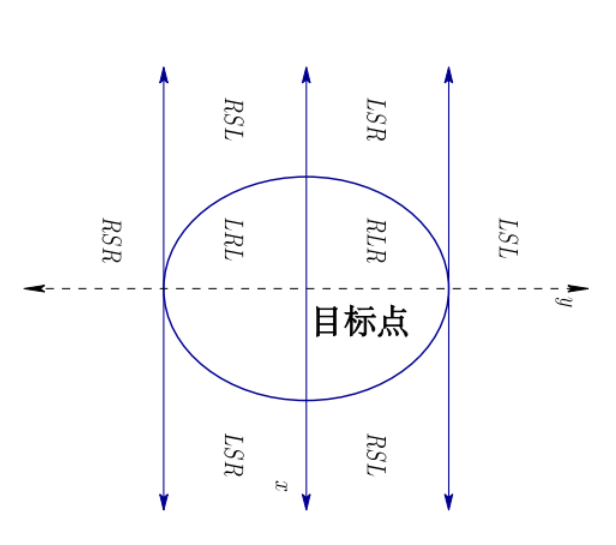
\includegraphics[width=0.43\textwidth]{images/DUBINSpi.png}
                                \caption{$\theta=\pi$时的单元分解情况}
                            \end{figure} 
                        \end{itemize}


                        \item \textbf{REEDS-SHEEP曲线}
                            \begin{figure}[H]
                                \centering
                                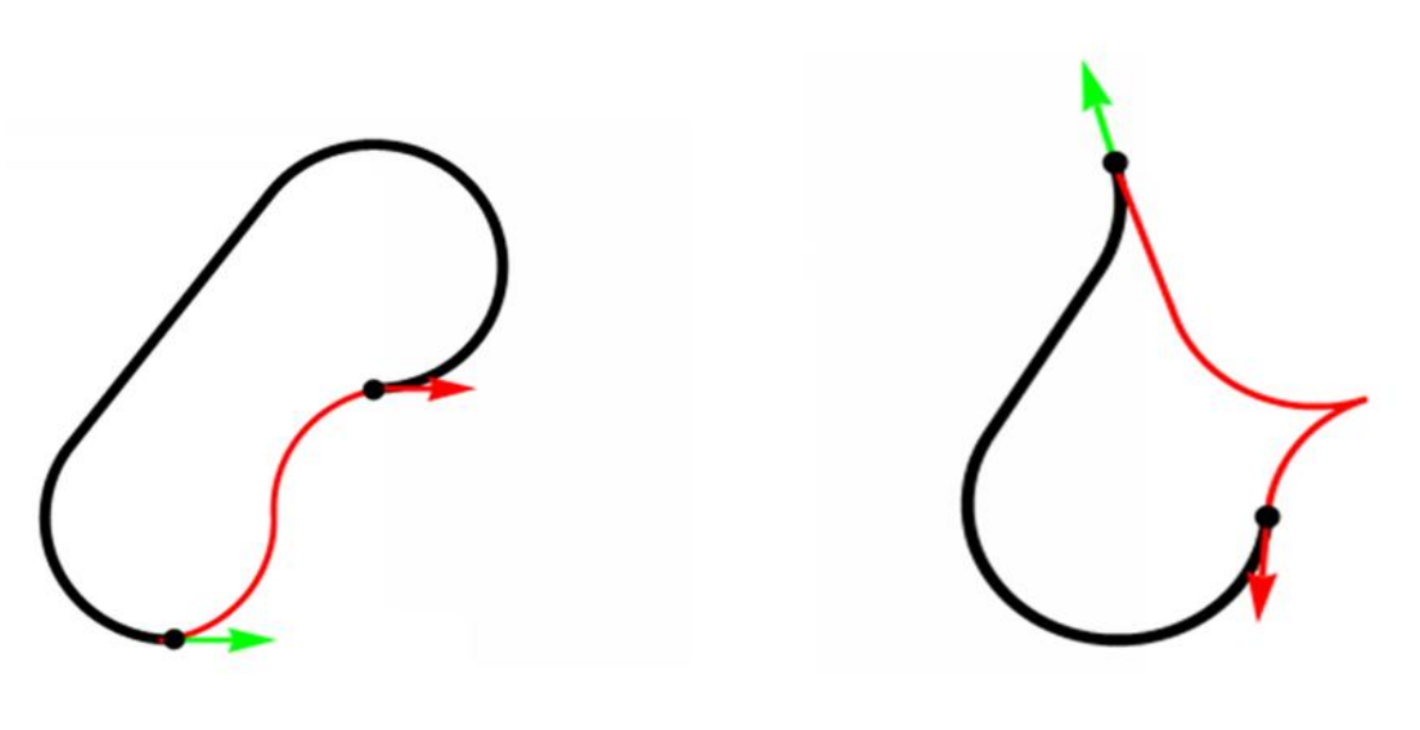
\includegraphics[width=0.43\textwidth]{images/reedssheep.png}
                                \caption{REEDS-SHEPP曲线}
                            \end{figure} 
                        \begin{itemize}
                            \item \textbf{系统方程}:\[
                            \quad
                            \begin{cases}
                            \dot{x} = u_1 \cos\theta, \\[4pt]
                            \dot{y} = u_1 \sin\theta, \\[4pt]
                            \dot{\theta} = u_1 u_2,
                            \end{cases}
                            \qquad
                            u_1 \in \{-1, 1\}, \quad
                            u_2 \in \left[-\dfrac{1}{L}\tan\phi_{\max},\; \dfrac{1}{L}\tan\phi_{\max}\right]
                            \]
                            \item \textbf{针对问题}:Dubins曲线中车辆只能向前运动,不能向后运动;本曲线可以向前也可以向后
                            \item \textbf{运动基元}:半径$\rho_{min}$向左(L)或者向右(R)转弯的圆弧以及直线(S),\textbf{引入新符号“|”},表示排挡运动,从向前运动切换到向后运动,或者从向后运动切换到向前运动
                            \item \textbf{最佳单词(48种)}:每个单词由\textbf{5个以下的运动基元组成},
                            \item \textbf{引入角度的单词}:\( \{ C\left| C\right| C,{CC}\left| {C,C}\right| {CC},{CSC},C{C}_{\beta }\left| {{C}_{\beta }C,C}\right| {C}_{\beta }{C}_{\beta }\left| {C,C}\right| {C}_{\pi /2}{SC}
                            \\,{CS}{C}_{\pi /2}\left| {C,C}\right| {C}_{\pi /2}S{C}_{\pi /2}|C\} \)
                            \\\small\kaishu{$C$指的是曲线,代替符号L和R;下标 \( \pi /2 \) 表示曲线必须精确地为 \( \pi /2 \) 的圆弧,下标$\beta$表示该运动基元参数必须和另一个运动基元参数匹配}
                        \end{itemize}
                    \end{enumerate}
                \end{itemize}
                    \item \textbf{参数优化法}\label{method:opt}
                        \begin{itemize}
                            \item \textbf{基本思想}:
                                \begin{enumerate}
                                    \item 对移动机器人参考点的速度控制律进行参数化表示
                                    \item 对速度控制量$v,\omega$单独规划控制
                                    \item 为满足起始点、终止点等位置边界约束,利用运动学和/或动力学模型合成各个速度控制量,得到速度控制的合成效果
                                    \item 根据合成效果和期望效果的差异,采用数值法在连续统中搜索得到满足边界条件的最优参数,确保满足空间位置约束
                                \end{enumerate}
                            \begin{figure}[H]
                                \centering
                                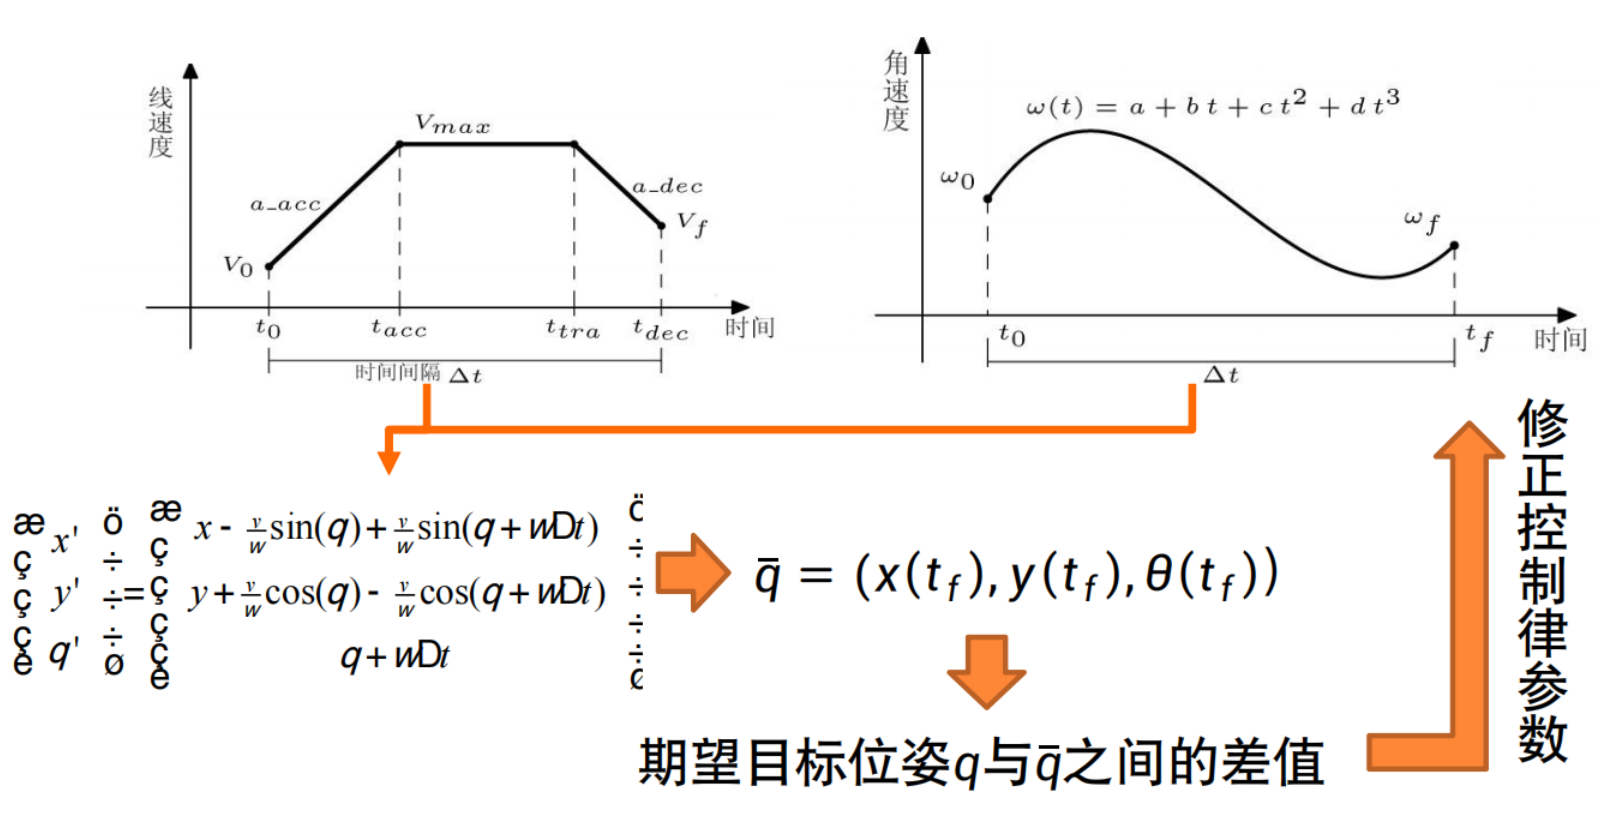
\includegraphics[width=0.85\textwidth]{images/canshuyouhuafa.png}
                                \caption{参数优化法的流程}
                            \end{figure} 
                            \item  \textbf{举例}:
                            \small\kaishu{
                            以上图为例,我们的速度和角速度的控制律分别是:
                            {
                            \[
                            v(t) = 
                            \begin{cases}
                            v_0 + a_a t, & t \in [t_0, T_a], \\[4pt]
                            v_c, & t \in [T_a, t_1 - T_d], \\[4pt]
                            v_1 - a_d (t_1 - t), & t \in [t_1 - T_d, t_1],
                            \end{cases}
                            \]
                            在这里我们需要确定的参数是$\Delta t$
                            \[
                            \omega(t) = a_0 + a_1 t + a_2 t^2 + a_3 t^3
                            \]
                            在这里我们需要确定的参数是$\Delta t,a_1,a_2,a_3$
                            \\因此,总的优化参数向量为\footnote{\small\kaishu
                            为什么只需要确定这些参数?\\[3pt]
                            (1)关于 $a_0$:它对应角速度多项式的初值项,通常由初始角速度条件(如 $\omega(0)=\omega_0$)直接给定,因此不需要优化,是已知量。\\[3pt]
                            (2)关于 $\Delta t$:它是整个轨迹的持续时间,直接影响线速度 $v(t)$ 与角速度 $\omega(t)$ 的积分结果(即位姿变化),故必须作为优化变量。\\[3pt]
                            (3)关于时间区间内部划分:各段时间区间 $[t_0,T_a]$、$[T_a,t_1-T_d]$、$[t_1-T_d,t_1]$ 通常根据加速度或最大速度约束自动确定;一旦 $\Delta t$ 被确定,这些分段时间点随之固定,因此不单独作为优化变量。
                            }:
                            \[
                            \mathbf{p} = 
                            \begin{bmatrix}
                            a_1 \\ a_2 \\ a_3 \\ \Delta t
                            \end{bmatrix}
                            \]
                        }   
                        \item \textbf{基本算法流程}\footnote{得到的是连续空间中的局部最优解,且求解效率与参数初值设置有很大关系}:
                        \begin{enumerate}
                        \item 设定参数的初值 $\mathbf{p}_0$,得到对应控制律\footnote{通常预先构造初始猜测查找表,或者构建神经网络建立边界约束与控制律参数之间的映射关系,根据边界约束要求找到表中最相邻的边界约束条件,以表中值作为初值,迭代计算得到最优控制律参数};
                        
                        \item 利用该控制律结合机器人运动学模型/动力学模型,可以计算得到在该控制律下机器人从初始状态运动达到的目标状态 $\bar{\mathbf{q}}_1$;
                        
                        \item 计算在控制律下到达的目标状态 $\bar{\mathbf{q}}_1$ 和期望目标状态 $\mathbf{q}_1$ 之间的误差 $\Delta \mathbf{q}$;
                        
                        \item 如果误差小于阈值,则结束,否则采用数值方法计算参数校正量 $\Delta \mathbf{p}$:
                        \[
                        \Delta \mathbf{p} = -\alpha \left[ \frac{\partial \Delta \mathbf{q}}{\partial \mathbf{p}} \right]^{-1}
                        \]
                        
                        \item 利用校正量校正参数值 $\mathbf{p}$,得到新的控制律,回到步骤2。
                        
                    \end{enumerate}}

                        \end{itemize}
                    \textbf{小结}:
                    \begin{table}[htbp]
                        \centering
                        \caption{图形搜索法与参数优化法比较}
                        \begin{tabular}{ccc}
                        \toprule
                        \textbf{比较内容} & \textbf{图形搜索法} & \textbf{参数优化法} \\
                        \midrule
                        控制量 & 位置 & 速度 \\
                        搜索空间连续性 & 离散 & 连续 \\
                        搜索结果最优性 & 全局最优 & 局部最优 \\
                        \bottomrule
                        \end{tabular}
                    \end{table}
                    \item \textbf{反馈控制法}\label{method:feedback}
                        \begin{itemize}
                            \item \textbf{基本思想}:根据当前状态与目标状态之间的差异,来生成减少这种差异的控制律
                            \item \textbf{优点}:
                                \begin{itemize}
                                    \item 简单,计算较快
                                    \item 参数意义明确,与效果直接对应
                                \end{itemize}
                            \item \textbf{缺点}:
                                \begin{itemize}
                                    \item 不考虑当前速度,容易造成速度不连续
                                    \item 平移速度、转向速度相互独立,但机器人总能力是有限的,且平移速度和转向速度存在关联
                                \end{itemize}
                            \item \textbf{计算流程}:\footnote{首先(a)到(d)推导平面机器人通用的,在平面内$v,\omega$与$\dot{\rho},\dot{\alpha},\dot{\beta}$即误差向量导数的关系,之后(e)设计控制律,代入控制律求解李雅普诺夫稳定性,使得该系统的平衡点是渐近稳定的,即误差会随着时间逐渐减小}
                            \begin{figure}[H]
                                \centering
                                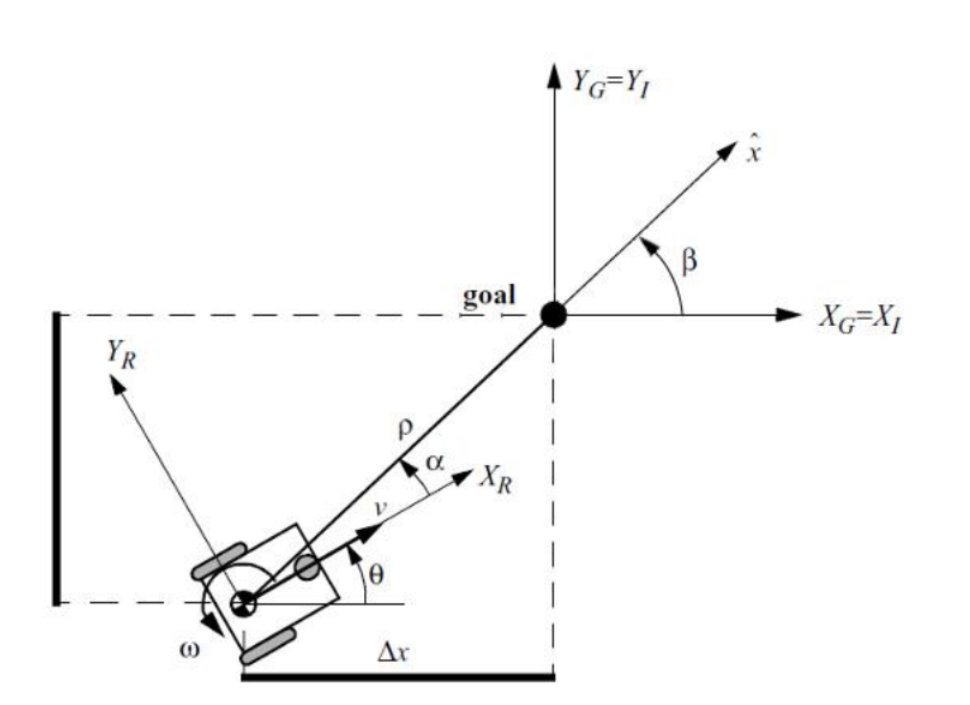
\includegraphics[width=0.35\textwidth]{images/feedbackcon.png}
                                \caption{反馈控制法坐标系图}
                            \end{figure} 
                            {\small\kaishu
                            \begin{enumerate}
                                \item \textbf{问题描述与目标}\\
                                机器人具有任意初始位姿与任意目标位姿。记当前位姿为
                                \[
                                \text{start} = 
                                \begin{bmatrix}
                                    x(t) \\ y(t) \\ \theta(t)
                                \end{bmatrix},
                                \quad
                                \text{goal} =
                                \begin{bmatrix}
                                    x_g \\ y_g \\ \theta_g
                                \end{bmatrix},
                                \]
                                实际姿态误差向量为
                                \[
                                \mathbf{e}(t) = \text{goal} - \text{start}.
                                \]
                                控制器设计的目标是寻找一个控制矩阵 $\mathbf{K}$,
                                生成机器人速度控制指令
                                \[
                                \begin{bmatrix}
                                    v(t) \\[2pt]
                                    w(t)
                                \end{bmatrix}
                                = \mathbf{K}\,\mathbf{e}(t),
                                \]
                                使误差趋向于零:
                                \[
                                \lim_{t \to \infty} \mathbf{e}(t) = \mathbf{0}.
                                \]
                            
                                \item \textbf{建立以目标为原点的坐标系}\\
                                不失一般性,设以目标位姿构建全局坐标系,目标点为坐标原点、目标朝向为 $x$ 轴。  
                                在该坐标系下,机器人运动学模型为:
                                \[
                                \begin{bmatrix}
                                    \dot{x} \\[2pt]
                                    \dot{y} \\[2pt]
                                    \dot{\theta}
                                \end{bmatrix}
                                =
                                \begin{bmatrix}
                                    \cos\theta & 0 \\[2pt]
                                    \sin\theta & 0 \\[2pt]
                                    0 & 1
                                \end{bmatrix}
                                \begin{bmatrix}
                                    v \\[2pt]
                                    w
                                \end{bmatrix}.
                                \]
                            
                                \item \textbf{从笛卡尔坐标到极坐标表示}\\
                                根据机器人与目标之间的距离与角度差定义误差:
                                \[
                                \Delta x = -x(t), \qquad
                                \Delta y = -y(t),
                                \]
                                \[
                                \rho = \sqrt{(\Delta x)^2 + (\Delta y)^2}, \qquad
                                \beta = \operatorname{atan2}(\Delta y, \Delta x), \qquad
                                \alpha = \beta - \theta.
                                \]
                                其中:
                                \begin{itemize}
                                    \item $\rho$ 表示机器人到目标的连线距离;
                                    \item $\beta$ 表示连线方向;
                                    \item $\alpha$ 表示车体朝向相对连线的夹角。
                                \end{itemize}
                            
                                \item \textbf{极坐标下的系统动力学}\\
                                \begin{itemize}
                                    \item 若 $\alpha \in (-\tfrac{\pi}{2}, \tfrac{\pi}{2}]$(车体朝向目标),则:
                                    \[
                                    \begin{bmatrix}
                                        \dot{\rho} \\[2pt] \dot{\alpha} \\[2pt] \dot{\beta}
                                    \end{bmatrix}
                                    =
                                    \begin{bmatrix}
                                        -\cos\alpha & 0 \\[4pt]
                                        \dfrac{\sin\alpha}{\rho} & -1 \\[8pt]
                                        \dfrac{\sin\alpha}{\rho} & 0
                                    \end{bmatrix}
                                    \begin{bmatrix}
                                        v \\[2pt] w
                                    \end{bmatrix}.
                                    \]
                                    \item 若 $\alpha \in (-\pi, -\tfrac{\pi}{2}] \cup (\tfrac{\pi}{2}, \pi]$(车体背向目标),则:
                                    \[
                                    \begin{bmatrix}
                                        \dot{\rho} \\[2pt] \dot{\alpha} \\[2pt] \dot{\beta}
                                    \end{bmatrix}
                                    =
                                    \begin{bmatrix}
                                        \phantom{-}\cos\alpha & 0 \\[4pt]
                                        -\dfrac{\sin\alpha}{\rho} & 1 \\[8pt]
                                        -\dfrac{\sin\alpha}{\rho} & 0
                                    \end{bmatrix}
                                    \begin{bmatrix}
                                        v \\[2pt] w
                                    \end{bmatrix},
                                    \qquad
                                    \text{在 } \rho = 0 \text{ 处存在奇异性}\footnote{\small\kaishu
                                    奇异性来源于 $\tfrac{\sin\alpha}{\rho}$ 项:当 $\rho \to 0$ 时除零导致方程不可定义,产生数值不稳定;
                                    实际表现为控制器在目标点附近振荡或发散。
                                    为消除奇异性,通常令 $v=k_\rho \rho$,
                                    使得 $\tfrac{v}{\rho}=k_\rho$ 成常数,从而闭环系统不再含 $1/\rho$,在 $\rho \to 0$ 时仍连续可微。}
                                    \]
                                \end{itemize}
                            
                                \item \textbf{控制律设计与奇异性消除}\\
                                取线性控制律:
                                \[
                                v = k_\rho \rho, \qquad w = k_\alpha \alpha + k_\beta \beta.
                                \]
                                代入情形 (a) 的系统方程,可得闭环系统:
                                \[
                                \dot{\rho} = -k_\rho \rho \cos\alpha, \qquad
                                \dot{\alpha} = k_\rho \sin\alpha - k_\alpha \alpha - k_\beta \beta, \qquad
                                \dot{\beta} = k_\rho \sin\alpha.
                                \]
                                此时由于 $\tfrac{v}{\rho}=k_\rho$ 为常数,$1/\rho$ 项被抵消,实现了奇异性消除
                            \end{enumerate}
                            }

                        \end{itemize}
            \end{enumerate}

\end{document}